\documentclass{beamer}
\mode<presentation>
\usepackage{amssymb,textcomp}
%\usepackage{beamerthemesplit}
\usepackage{beamerthemeJuanLesPins}
\usepackage{verbatim}
\usepackage{algorithm2e}
\usefonttheme{serif}
\title{Unidad III: Aproximaci\'on de funciones.}
\author{Jos\'e Luis Ram\'irez B.}
\date{\today}

\begin{document}

\frame{\titlepage}

\frame{\tableofcontents}

\section{Introducci\'on}
\begin{frame}[fragile]
  \frametitle{Motivaci\'on.} 
  \begin{itemize}
   \item<1-> En este tema se da una posible respuesta a una situaci\'on
bastante natural en el \'ambito cient\'ifico.
    \item<2-> Se Investiga un fen\'omeno que se est\'a desarrollando, se desea estudiarlo, y junto
con los modelos previos con que se cuente, se pueden tomar
muestras experimentales.
    \item<3-> Se tiene una serie de datos a partir de
mediciones sobre el mismo.
    \item<4-> Se desea extraer informaci\'on de esos datos.
  \end{itemize}
\end{frame}
%%%%%
\begin{frame}[fragile]
  \frametitle{Motivaci\'on.}
  Esencialmente podemos tratarlo con:
\begin{itemize}
 \item<2-> T\'ecnicas estad\'isticas (que continuar\'an observando el fen\'omeno de un modo discreto, es decir, sobre ese conjunto finito de mediciones).
 \item<3-> o bien ``intentando recrear/reconstruir el fen\'omeno en su totalidad'' (en un dominio continuo de espacio, tiempo o cualquier otra magnitud), con la funci\'on que represente ``lo mejor posible'' esos datos.
\end{itemize}
\end{frame}
%%%%%
%%%%
\frame
{
  \frametitle{Motivaci\'on.}
Las t\'ecnicas que utilizan funciones continuas y se consideran en este curso son de dos tipos:
\begin{itemize}
 \item<2-> Interpolaci\'on: c\'alculo de funciones que pasan (``interpolan'' es el t\'ermino matem\'atico) exactamente por los puntos dados.
 \item<3-> Curvas de ajuste: c\'alculo de funciones aproximadas a los datos que tenemos (en alg\'un sentido, para cierta distancia)
\end{itemize}
}
%%%%%
\frame{
%\footnotesize
\frametitle{Resultados Fundamentales}
\begin{block}{Polinomio de grado $n$:}
 $$p_n(x)=a_nx^n+a_{n-1}x^{n-1}+\cdots+a_1x+a_0\,(a_n \neq 0)$$
\end{block}
 
\uncover<2->
{\begin{block}{Teorema:}
Si $p_n$ es un polinomio de grado $n \geq 1$, entonces $p_n(x) = 0$ tiene al menos una ra\'iz (posiblemente compleja).
\end{block}}
}
%%%
\frame{
  \frametitle{Resultados Fundamentales}
\uncover<1->{
\begin{block}{Teorema:}
Sea $p_n$ un polinomio de grado $n \geq 1$, entonces existen constantes $x_1, x_2,\ldots,x_k$, posiblemente complejas, y enteros positivos $m_1, m_2, \ldots, m_k$, tales que $m_1 + m_2 + \ldots + m_k = n$ verificando:
$$
p_n(x) = a_n(x - x_1)^{m_1}(x - x_2)^{m_2}\cdots(x - x_k)^{m_k}
$$
\end{block}}
\uncover<2->{
\begin{block}{Teorema:}
Sean $p_n$ y $q_n$ dos polinomios de grado menor o igual que $n$. Si existen $x_1, x_2, \ldots, x_k,$ con $k > n$, n\'umeros distintos tales que $p_n(x_i) = q_n(x_i)$, $i = 1,\ldots , k$, entonces $p_n(x) = q_n(x)$ para todo $x$.
\end{block}}
}
%%%%
%%%%
\frame{  
\frametitle{Evaluaci\'on de polinomios}
\vspace{-0.5cm}
\footnotesize{
\begin{block}{$p_n(x)=a_nx^n+a_{n-1}x^{n-1}+\cdots+a_1x+a_0$}
Se necesitan menos operaciones para evaluarlo en un punto $x_0$ si se escribe:
$$
p_n(x) = a_0 + x(a_1 + x(\cdots(a_{n-2} + x(a_{n-1} + xa_n))\cdots))
$$
\end{block}}

\footnotesize{
\begin{block}{Algoritmo de Horner para evaluar $p_n(x_0)$}
\uncover<2->{
$$
\begin{array}{lr}
b_{n-1} = a_n\\
b_k = a_{k+1}+x_0b_{k+1} & k=n-2,\ldots,1,0,-1
\end{array}
$$
entonces: $p_n(x_0) = b_{-1}$}

\uncover<3->{
Adem\'as, si se llama
$$
q_{n-1}(x) = b_{n-1}x^{n-1}+b_{n-2}x^{n-2}+\cdots+b_1x+b_0
$$
se tiene que:
$$
p_n(x) = (x-x_0)q_{n-1}(x)+b_{-1}
$$
y por lo tanto
$$
p'_n(x_0) = q_{n-1}(x_0)
$$}
\end{block}}
}
%%%%
\frame{
\frametitle{Evaluaci\'on de polinomios}
\textquestiondown Por qu\'e es Importante el Algoritmo de Horner?
\begin{itemize}
 \item<2-> Eficiencia: Es m\'as eficiente que calcular las potencias de 
 $x_0$ y multiplicar por los coeficientes de forma individual (se usa 
 menos memoria y tiempo de c\'omputo).
 \item<3-> Estabilidad: Reduce errores de redondeo en c\'alculos num\'ericos.
 \item<4-> Derivadas: Permite obtener informaci\'on sobre la derivada del polinomio 
 en el mismo punto.
 \item<5-> Divisi\'on Sint\'etica: Est\'a relacionado con el m\'etodo de divisi\'on sint\'etica
 para polinomios, lo que lo hace muy \'util en el campo del \'algebra y el an\'alisis num\'erico.
\end{itemize}
}
%%%%
\frame{
\frametitle{Evaluaci\'on de polinomios}
En Resumen:
\begin{itemize}
\item El algoritmo de Horner es una herramienta poderosa para evaluar polinomios y 
tambi\'en para obtener informaci\'on sobre su derivada.
\item Es un m\'etodo eficiente, estable y muy utilizado en diversos campos de las matem\'aticas y la inform\'atica.
\end{itemize} 
}
%%%%%
\frame{
\frametitle{Ejemplo: Polinomio de Grado 3}

Tenemos el polinomio:
$$
p_3(x) = 2x^3 - 3x^2 + 4x - 1
$$
Y queremos evaluarlo en $x_0 = 2$ y tambi\'en calcular $p'_3(2)$.
}
\frame{
\frametitle{Ejemplo: Polinomio de Grado 3}
\begin{enumerate}
\item[1.] Aplicaci\'on del Algoritmo de Horner para $p_3(2)$

Recordemos que el algoritmo es:
\begin{block}{}
$$
\begin{array}{l}  
b_{n-1} = a_n\\
b_k = a_{k+1} + x_0 \cdot b_{k+1} \text{ para }k = n-2, ..., 1, 0, -1\\
p_n(x_0) = b_{-1}
\end{array}
$$
\end{block}
\begin{itemize}
  \item<2-> Inicializaci\'on:\\
$b_2 = a_3 = 2$ (coeficiente de $x^3$)
\item<3-> Iteraci\'on:\\
$b_1 = a_2 + x_0 \cdot b_2 = -3 + 2 \cdot 2 = 1$ (coeficiente de $x^2$)\\
$b_0 = a_1 + x_0 \cdot b_1 = 4 + 2 \cdot 1 = 6$ (coeficiente de $x^1$)\\
$b_{-1} = a_0 + x_0 \cdot b_0 = -1 + 2 \cdot 6 = 11$ (t\'ermino independiente)
\item<4-> Resultado:\\
$p_3(2) = b_{-1} = 11$
\end{itemize}
\end{enumerate}
}
%%%%%
\frame{
\frametitle{Ejemplo: Polinomio de Grado 3}
\begin{enumerate}
\item[2.] Obtención del Polinomio Cociente $q_2(x)$\\
Con los valores de $b$ que obtuvimos (excepto $b_{-1}$), podemos formar el polinomio cociente de grado 2:
$$
q_2(x) = b_2 x^2 + b_1 x + b_0 = 2x^2 + 1x + 6
$$
\item[3.]<2-> Relaci\'on entre $p_3(x)$, $q_2(x)$ y $b_{-1}$\\
El polinomio $p_3(x)$ se puede expresar como:\\
$p_3(x) = (x - x_0) \cdot q_2(x) + b_{-1}$\\
$p_3(x) = (x - 2) \cdot (2x^2 + x + 6) + 11$
\end{enumerate}
}
%%%%%
\frame{
\frametitle{Ejemplo: Polinomio de Grado 3}
\begin{enumerate}
\item[4.]<1-> Aplicaci\'on del Algoritmo de Horner a $q_2(x)$ para obtener $q_2(2) = p'_3(2)$

Aplicando el algoritmo de Horner para evaluar el polinomio $q_2(x)$ en $x_0 = 2$. Los coeficientes de $q_2(x)$ son: $b_2=2$, $b_1=1$, $b_0=6$

Llamemos a los nuevos coeficientes $c_i$:
\begin{itemize}
\item<2->Inicializaci\'on:\\
$c_1 = b_2 = 2$
\item<3->Iteraci\'on:\\
$c_0 = b_1 + x_0 \cdot c_1 = 1 + 2 \cdot 2 = 5$\\
$c_{-1} = b_0 + x_0 \cdot c_0 = 6 + 2 \cdot 5 = 16$
\item<4-> Resultado:\\
$q_2(2) = c_{-1} = 16$
\end{itemize}
\end{enumerate}
}
%%%%
\frame{
\frametitle{Ejemplo: Polinomio de Grado 3}
\begin{enumerate}
\item[5.]<1-> Derivada $p'_3(2)$\\
Se tiene que\\
$p'_3(2) = q_2(2) = 16$
\end{enumerate}
En resumen:
\begin{itemize}
\item<2-> $p_3(2) = 11$
\item<3-> $q_2(x) = 2x^2 + x + 6$
\item<4-> $p_3(x) = (x - 2) * (2x^2 + x + 6) + 11$
\item<5-> $p'_3(2) = q_2(2) = 16$
\end{itemize}
}
%%%%%
\frame{
\frametitle{Ejemplo: Polinomio de Grado 3}
{\bf Comprobaci\'on de la Derivada}

Derivando el polinomio $p_3(x)$ y evalu\'andolo en $x = 2$.
\begin{block}{}
$$
\begin{array}{l}
p_3(x) = 2x^3 - 3x^2 + 4x - 1\\
p'_3(x) = 6x^2 - 6x + 4
\end{array}
$$
\end{block}
\uncover<2->{
Evaluando en x = 2:
$$
p'_3(2) = 6(2^2) - 6(2) + 4 = 6(4) - 12 + 4 = 24 - 12 + 4 = 16
$$
}
}
%%%%
\section{Interpolaci\'on}
\subsection{Taylor}
\frame{
\frametitle{Problema de interpolaci\'on de Taylor}
\uncover<1->
{
\begin{block}{Problema de interpolaci\'on de Taylor}
Dados un entero $n$ no negativo, un punto $x_0 \in \mathbb{R}$ y los valores $f(x_0),f'(x_0),\ldots,f^{(n)}(x_0)$ de una funci\'on y sus $n$ primeras derivadas en $x_0$, encontrar un polinomio $P(x)$ de grado $\leq n$ tal que
$$
P(x_0) = f(x_0), P'(x_0) = f'(x_0),\ldots, P^{(n)}(x_0) = f^{(n)}(x_0).
$$
\end{block}}
\uncover<2->{
\begin{block}{Teorema:}
El problema de interpolaci\'on de Taylor tiene soluci\'on \'unica, que se denomina polinomio de Taylor de grado $\leq n$ de la funci\'on $f$ en el punto $x_0$:
\[
\textstyle
P(x) = f(x_0)+f'(x_0)(x-x_0)+f''(x_0)\frac{(x-x_0)^2}{2!}+\cdots+f^{(n)}(x_0)\frac{(x-x_0)^n}{n!}
\]
\end{block}}
}
%%%%
\frame{
\frametitle{Problema de interpolaci\'on de Taylor}
\uncover<1->{
\begin{block}{Teorema:}
Para $n > 1$ sea $f(x)$ una funci\'on $n$ veces derivable en $x_0$. El polinomio de Taylor $P(x)$ verifica que:
$$
\lim_{x \to x_0}\frac{f(x)-P(x)}{(x-x_0)^n}=0
$$
con la notaci\'on $o$ peque\~na de Landau $f(x) - P(x) = o((x - x_0)^n)$ para $x \to x_0$. Adem\'as, $P(x)$ es el \'unico polinomio de grado $\leq n$ con esta propiedad.
\end{block}}
}
%%%%
\frame{
\frametitle{Problema de interpolaci\'on de Taylor}
\begin{itemize}
 \item Error del polinomio interpolador de Taylor
\uncover<2->{
\begin{block}{Teorema:}
Sean $x$ y $x_0$ dos n\'umeros reales distintos y $f(x)$ una funci\'on con $n$ derivadas continuas en un intervalo conteniendo a $x$ y $x_0$, en el que tambi\'en existe $f^{(n+1)}$. Entonces existe un punto $\xi$ entre $x$ y $x_0$ tal que:
$$
f(x)-P(x) = f^{(n+1)}(\xi)\frac{(x-x_0)^{n+1}}{(n+1)!}
$$
\end{block}}
\end{itemize}
}
%%%%
\frame{
\frametitle{Problema de interpolaci\'on de Taylor}
\begin{block}{Colorario:}
Adem\'as de las hip\'otesis del teorema supongase que para cada $t$ entre $x$ y $x_0$ se verifica que $|f^{(n+1)}(t)| \leq K_{n+1}$ constante, entonces:
$$
|f(x)-P(x)| \leq \frac{|x-x_0|^{(n+1)}K_{n+1}}{(n+1)!}
$$
\end{block}
}
%%%%
\frame{
\frametitle{Ejemplo:}
A continuaci\'on se muestran las gr\'aficas de la funci\'on $f(x) = \sin(x)$ y de su polinomio de Taylor de orden 1 al 9 en el cero. Se puede comprobar que la aproximaci\'on es m\'as exacta a medida que se aumenta el orden.
\begin{center}
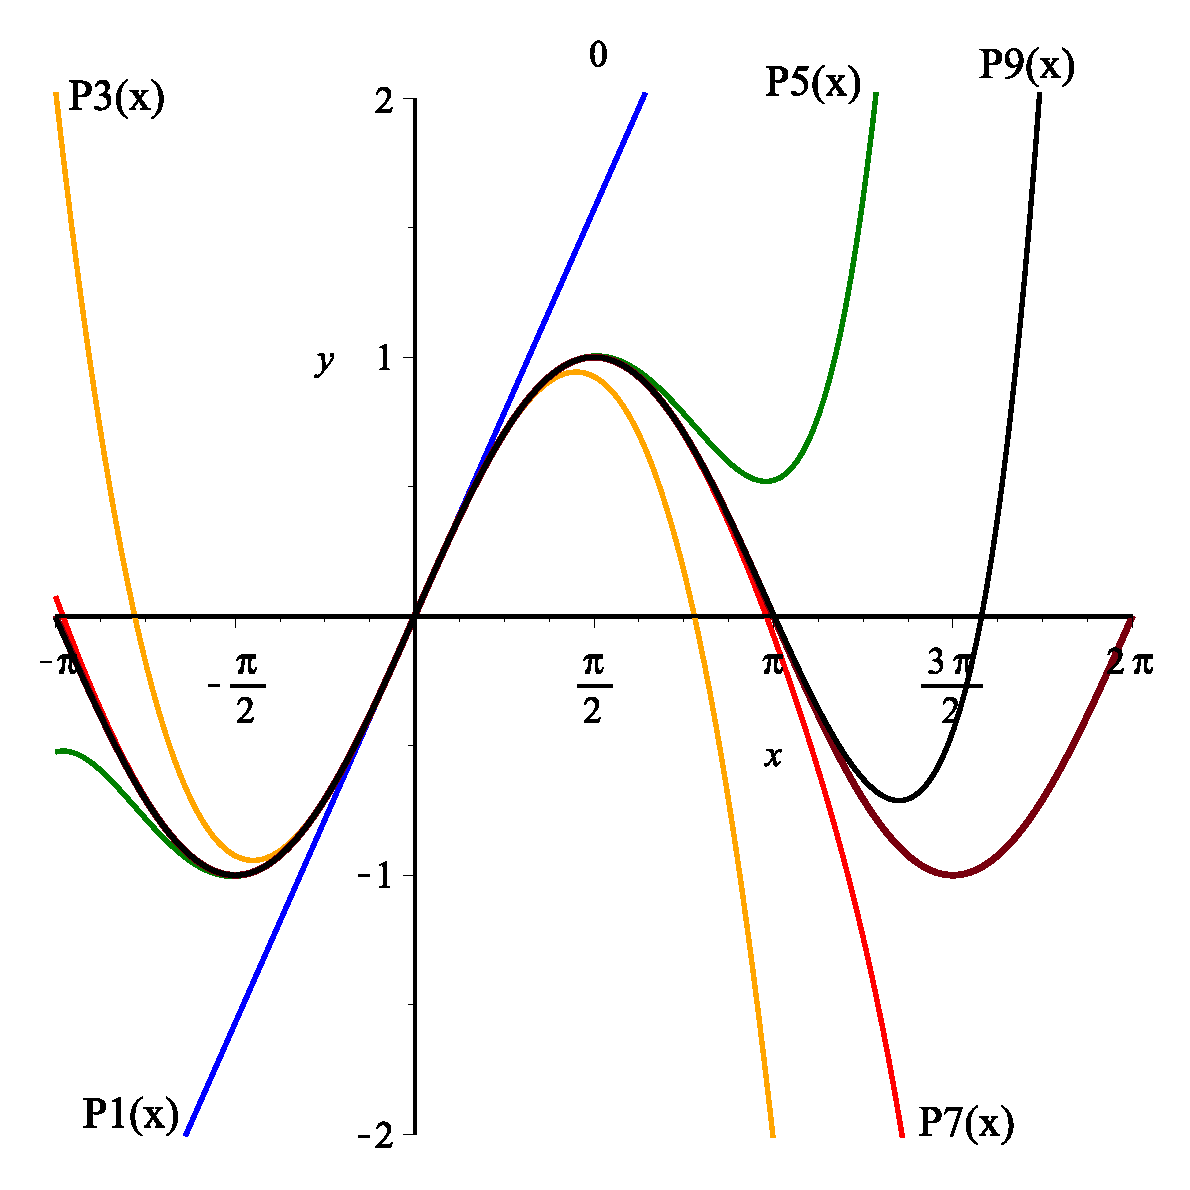
\includegraphics[scale=0.28]{taylorsin.eps}
\end{center}
}
%%%%
\frame{
\frametitle{Ejemplo:}
El hecho de que la funci\'on seno y su polinomio de Taylor se parezcan tanto como se quiera, con s\'olo aumentar el grado del polinomio lo suficiente, no es algo que le ocurra a todas las funciones. Para la funci\'on arctan la situaci\'on no es tan buena:
\begin{center}
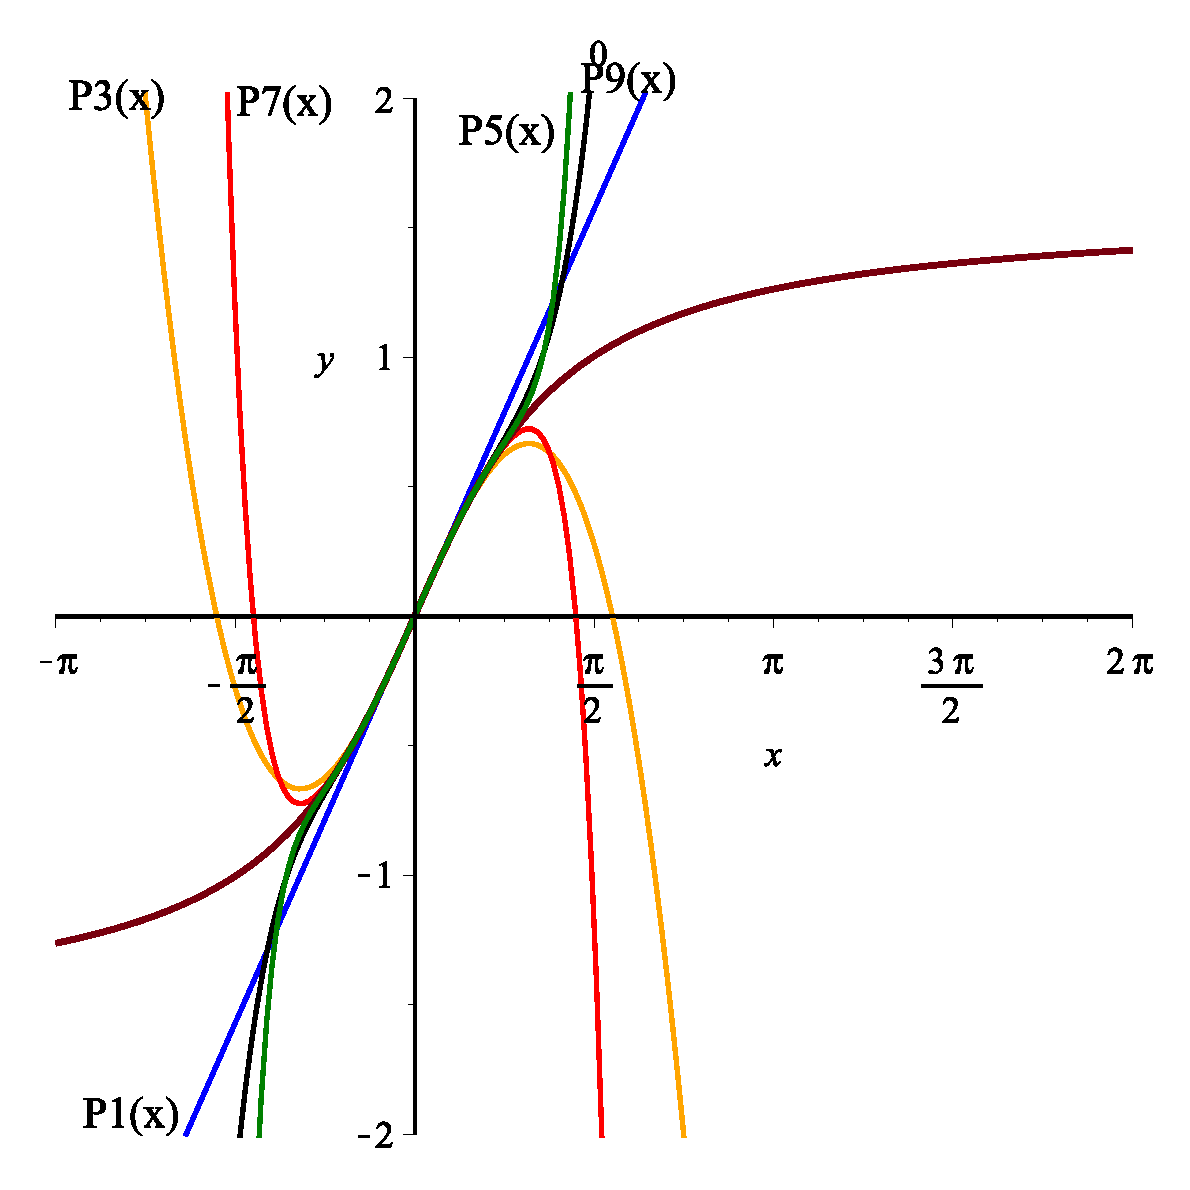
\includegraphics[scale=0.28]{tayloratan.eps}
\end{center}
}
%%%%%
\begin{frame}
  \frametitle{Ejemplo:}
  \begin{itemize}
    \item Se  desea aproximar la funci\'on $f(x)=e^x$ mediante el polinomio de Taylor centrado en $x_0=0$ de orden 5 y hallar el error obtenido en la estimaci\'on para $x=1.5$ 
   
    \item El polinomio de Taylor de grado 5 viene dada por la siguiente expresi\'on
    \begin{block}{}
    \scriptsize{
    $$
    \begin{array}{c}
      P_5(x) = 1+1(x-0)+\dfrac{1}{2!}(x-0)^2+\dfrac{1}{3!}(x-0)^3+\dfrac{1}{4!}(x-0)^4+\dfrac{1}{5!}(x-0)^5\\[10pt]
      P_5(x) = 1+x+\dfrac{1}{2!}x^2+\dfrac{1}{3!}x^3+\dfrac{1}{4!}(x-0)^4+\dfrac{1}{5!}x^5
    \end{array}
    $$}
    \end{block}
  \end{itemize}
\end{frame}
%%%%%
\begin{frame}
  \frametitle[short title]{Ejemplo:}
  Con la expresi\'on del residuo se calcula el error de Truncamiento:
  \begin{block}{}
    $$
    R_5(x) = \dfrac{f^{(6)}(\xi)}{6!}(x-x_0)^6=\dfrac{f^{(6)}(\xi)}{6!}x^6 = \dfrac{e^\xi}{6!}x^6
    $$
    $$
    R_5(x)=\dfrac{e^\xi}{6!}x^6
    $$
  \end{block}
\end{frame}
%%%%%
\begin{frame}
\frametitle{Ejemplo:}
 \begin{itemize}
   \item Ahora, vamos a aproximar $f(1.5) = e^{1.5}$ usando $P_5(1.5)$:\\
   $P_5(1.5) = 1 + 1.5 + \dfrac{(1.5)^2}{2} + \dfrac{(1.5)^3}{6} + \dfrac{(1.5)^4}{24} + \dfrac{(1.5)^5}{120}$
 \item<2-> Obtenemos:\\
   $P_5(1.5) \approx 4.462$
 \item<3-> C\'alculo del error en $x = 1.5$\\
 El error en la aproximaci\'on de Taylor est\'a dado por el t\'ermino del resto. La forma del resto para el polinomio de Taylor de orden $n$ es:\\
 $$
 R_n(x) = \dfrac{f^{(n+1)}(\xi)}{(n+1)!}(x-x_0)^{n+1}
 $$ 
 \end{itemize}
\end{frame}
%%%%%
\begin{frame}
\frametitle{Ejemplo:}
 \begin{itemize}
   \item<1-> En nuestro caso, $n = 5$, $x = 1.5$, $x_0 = 0$, y la derivada de orden 6 (o cualquiera) de $e^x$ es $e^x$.\\
   Por lo tanto:
   $$
   \begin{array}{l}
   R_5(1.5) = \dfrac{e^\xi \cdot (1.5 - 0)^6}{6!}\\[10pt]
   R_5(1.5) = \dfrac{e^\xi \cdot 1.5^6}{720} 
   \end{array}
   $$
   Donde $\xi$ es un n\'umero entre 0 y 1.5.
   \item<2-> Para maximizar el error, tomamos el mayor valor posible de $e^\xi$ en el intervalo [0, 1.5]. Este valor es cuando $c=1.5$.\\
Por lo tanto
$$
R_5(1.5) = e^{1.5} \cdot \dfrac{(1.5)^6}{720} \approx 0.0708
$$
 \end{itemize}
\end{frame}
%%%%
\frame{
\frametitle{Ejemplo:}
 \begin{itemize}
   \item<1-> C\'alculo del Valor Real y el Error Exacto

   \item<2-> El valor real de $e^{1.5}$ es aproximadamente 4.481689.
   
   \item<3-> El error exacto es:
   $$
   \begin{array}{l}
   \text{Error} = |e^{1.5} - P_5(1.5)|\\[10pt]
   \text{Error} = |4.481689 - 4.462 |\\[10pt]
   \text{Error} = 0.019689
   \end{array}
   $$
  \end{itemize}
}
%%%%
\subsection{Lagrange}
\frame
{
\frametitle{Interpolaci\'on}
\begin{itemize}
 \item<1-> Nos centraremos ahora en el problema de obtener, a partir de una tabla de parejas $(x,f(x))$ definida en un cierto intervalo $[a,b]$, el valor de la funci\'on para cualquier $x$ perteneciente a dicho intervalo.
 
 \item<2-> Supongamos que se dispone de las siguientes parejas de datos:
$$
\begin{array}{|c|c|c|c|c|c|}\hline
  \textbf{x} & x_0 & x_1 & x_2 & \cdots & x_n\\\hline
  \textbf{y} & y_0 & y_1 & y_2 & \cdots & y_n\\\hline
 \end{array}
$$
\end{itemize}
}
%%%%
\frame
{
  \begin{itemize}
    \item El objetivo es hallar una funci\'on continua lo m\'as sencilla posible tal que:
    \begin{block}{}
    $$
      \widetilde{f}(x_k) = y_k = f(x_k) \quad\forall k = 0,\ldots,n
    $$
    \end{block}
    en donde $x_k$ y $f(x_k)$ son datos conocidos.

    \item<2->Se dice entonces que la funci\'on $\widetilde{f}(x)$ , es una funci\'on interpolante de los datos representados en la tabla.
    \uncover<3->{\begin{block}{Observaci\'on:}
      En general, trabajaremos con $f$ = polinomios de grado $\leq n$
      $$
      P(x) = a_nx^n + a_{n-1}x^{n-1} + \cdots + a_1x + a_0
      $$
      polinomio algebraico
      \end{block}}
\end{itemize}
}
%%%%
\frame
{
\begin{figure}
 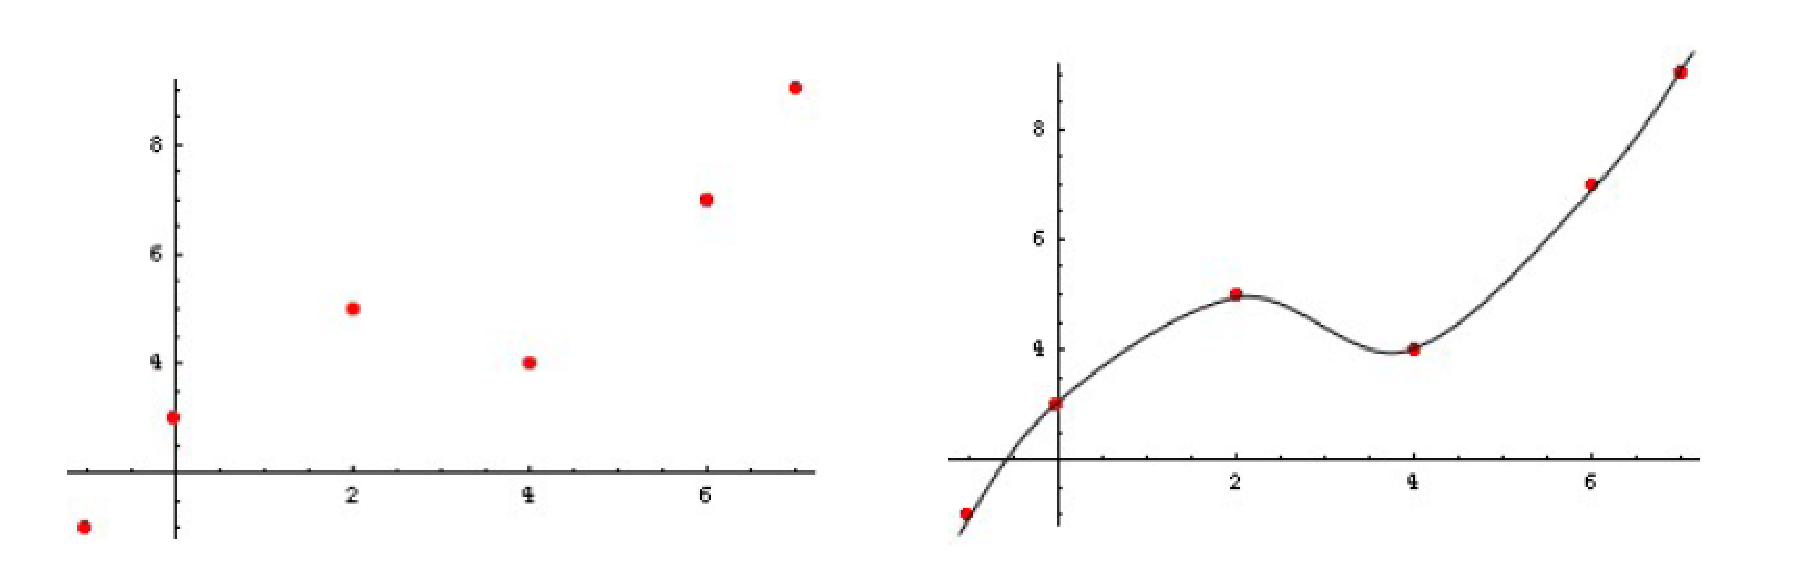
\includegraphics[scale=0.37]{img1.eps}
 \caption{Datos de iterpolaci\'on y curva interpolante.}
\end{figure}
}
%%%
\frame
{
\begin{block}{Teorema de Weierstrass:}
Sea $f$ continua sobre $[a,b]$, dado $\varepsilon > 0 \quad \exists P(x)$ polinomio tal que $\mid f(x)-P(x)\mid < \varepsilon \quad \forall x\in [a,b]$.
\end{block}
}
%%%%%
\frame
{
\frametitle{Polinomio interpolador de Lagrange}
\begin{itemize}
\item Si se escribe $P(x) = a_0 + a_1x + \cdots + a_nx^n$. As\'i, $P(x)$ ser\'a soluci\'on del problema si, y s\'olo si, el S.E.L:
\begin{block}{}
$$
\left(
\begin{array}{ccccc}
 1 & x_0 & x_0^2 & \cdots & x_0^n\\
 1 & x_1 & x_1^2 & \cdots & x_1^n\\
 1 & x_2 & x_2^2 & \cdots & x_2^n\\
 1 & \vdots & \vdots & \ddots & \vdots\\
 1 & x_n & x_n^2 & \cdots & x_n^n\\
\end{array}\right)
\left(
\begin{array}{c}
 a_0\\
 a_1\\
 a_2\\
 \vdots\\
 a_n\\
\end{array}\right) =
\left(
\begin{array}{c}
 y_0\\
 y_1\\
 y_2\\
 \vdots\\
 y_n\\
\end{array}
\right)
$$
\end{block}
admite soluci\'on.

\item<2-> que se denomina sistema cuadrado de Vandermonde. La matriz $A$ del sistema se denomina matriz de Vandermonde y es no-singular si los puntos $x_0, x_1, \ldots , x_n$ son diferentes. Esta matriz es mal condicionada a medida que $n$ aumenta.
\end{itemize}
}
%%%%%
\begin{frame}
  \frametitle{Polinomio interpolador de Lagrange}
  \begin{itemize}
    \item Llamando $A$ a la matriz de coeficientes del sistema; se tiene que el problema de interpolaci\'on admite una \'unica soluci\'on si, y s\'olo si, los nodos de interpolaci\'on son distintos. Para ello basta con probar que $\det(A) = \prod_{i>j}(x_i-x_j)$ y, por lo tanto, $\det(A) \neq 0 \Leftrightarrow x_i \neq x_j$.
    \item<2-> El m\'etodo de Lagrange para interpolaci\'on polinomial resulta de resolver este sistema para obtener los coeficientes pero lo hace de una forma m\'as sencilla y sistem\'atica. 
  \end{itemize}
\end{frame}
%%%%%
\frame{
\frametitle{Interpolaci\'on de Lagrange}
Para calcular el polinomio interpolador $P(x)$ asociado a una tabla de datos $(x_i, y_i)$ con $i =0,\ldots,n$ se puede plantear una simplificaci\'on previa: se construyen polinomios $l_i(x)$ de grado $n$ que valgan 1 en el nodo $x_i$ y 0 en el resto.

\begin{block}{}
$$
l_i(x_k) = \delta_{ik}=\left\{
\begin{array}{ccc}
 1 & \textrm{si} & i=k\\
 0 & \textrm{si} & i\neq k
\end{array}
\right.
$$
\end{block}
\uncover<2->{Si se escribe el polinomio factorizado para que tenga en
cada nodo $x_j$ (con $j \neq i$) una ra\'iz, el candidato es:
\begin{block}{}
$$
(x - x_0)(x - x_1)\cdots (x - x_{i-1})(x - x_{i+1}) \cdots (x - x_n) = \prod_{j=0,j\neq i}^n(x - x_j)
$$
\end{block}}
}
%%%
\frame
{\frametitle{Polinomio interpolador de Lagrange}
Lo \'unico que no se consigue es que en $x_i$ valga 1, para ello hay que ``normalizar'' la funci\'on anterior.

\uncover<2->{As\'i, finalmente la f\'ormula de interpolaci\'on de Lagrange es:
\begin{block}{}
$$
P(x) = \sum_{k=0}^n y_kl_k(x), \quad l_k(x) = \prod_{j=0,j\neq k}^n\frac{x - x_j}{x_k - x_j}, k=0,\ldots,n
$$
\end{block}
Los polinomios $l_k(x)$ reciben el nombre de polinomios de Lagrange.}
}
%%%%%
\begin{frame}
  \frametitle{Interpolaci\'on de Lagrange}
\begin{block}{Teorema:}
  Sean $x_0, x_1, \ldots , x_n$, $n + 1$ n\'umeros diferentes, y sea $f$ una funci\'on tal que
sus valores se obtengan a partir de los n\'umeros dados $(f(x_0), f(x_1), \ldots , f(x_n))$, entonces
existe un \'unico polinomio $p_n(x)$ de grado $n$, que cumple con la propiedad
$$
f(x_k) = p_n(x_k) \text{ para cada }k = 0,1, \ldots , n
$$
y este polinomio est\'a dado por la siguiente expresi\'on
\small{
$$
p_n(x) = f(x_0)L_0(x) + f(x_1)L_1(x) + \cdots + f(x_n)L_n(x) = \sum_{k=0}^nf(x_k)L_k(x)
$$}
\end{block}
\end{frame}
%%%%%
\begin{frame}
  \frametitle{Interpolaci\'on de Lagrange}
  Demostraci\'on:
  \begin{itemize}
    \item Se tiene que $p_n(x)=L_0(x)f(x_0)+L_1(x)f(x_1)+\cdots+L_n(x)f(x_n)$ ya que $L_k(x)$ 
    son polinomios de grado menor o igual a $n$ esto implica que $p(x)$ es un polinomio de grado menor o igual a $n$.
    \item<2-> Adem\'as
    $$
    \begin{array}{l}
    L_k(x_k) = 1,\quad L_k(x_j) =0 \mbox{ si $j \neq k$}\\
    \text{\small $\Rightarrow p_n(x_k) = 0 + 0 + \cdots + f(x_k) + \cdots + 0 = f(x_k) \quad \forall k=0,1,\ldots,n$}
    \end{array}
    $$
  \end{itemize}
\end{frame}
%%%%%
\begin{frame}
  \frametitle{Interpolaci\'on de Lagrange}
  \begin{itemize}
    \item La unicidad puede demostrarse como sigue:
    
    \item<2-> Supongase que $p_n(x)$ y $q_n(x)$ son dos polinomios de grado $\leq n$ que interpolan a $f(x)$ en los $n+1$ 
    puntos distintos $x_k,\quad k = 0,\ldots, n$, es decir
    $$
    p_n(x_k) = q_n(x_k) = f(x_k), \qquad k=0,1 \ldots,n
    $$
    \uncover<3->{
    Entonces, $r_n(x) = p_n(x)-q_n(x)$ es un polinomio de grado $\leq n$ con $n+1$ raices $x_0, x_1, \ldots, x_n$. Pero cualquier polinomio de grado $n$ con un n\'umero de raices mayor a $n$ debe ser constante e igual a cero. Por lo tanto $r_n (x) \equiv 0, \forall x$, y en consecuencia $p_n (x) = q_n (x), \forall x \in [a, b]$.}
  \end{itemize}
\end{frame}
%%%%
\frame
{
\frametitle{Polinomio interpolador de Lagrange}
Si $x_0,\ldots,x_n$ son $n+1$ n\'umeros reales distintos y $f$ es una funci\'on real definida sobre ellos, entonces existe un \'unico polinomio $P_n(x)$ de grado menor o igual a $n$ tal que
$f(x_k)=P(x_k)\quad \forall k=0,\ldots,n$.

\uncover<2->{
  \begin{block}{Teorema}
  
    Si $f \in \mathcal{C}^{n+1} [a, b]$ y $p_n(x)$ es el polinomio de interpolaci\'on en $n+1$ puntos distintos $x_0 = a, 
    x_1 , \ldots , x_n = b$, entonces para cada $x \in [a, b]$ existe $\xi(x) \in I[x_0 , x_1 , . . . , x_n , x]$ (el 
    intervalo cerrado m\'as peque\~no que contiene $x_0 , x_1 , \ldots , x_n , x$) tal que
    $$
   f(x) - p_n(x) = \dfrac{f^{(n+1)}(\xi(x))}{(n+1)!}w(x) \qquad \mbox{con } w(x) = \prod_{j=0}^n(x-x_j)
   $$
   \end{block}
}
}
%%%%%%
\frame{
  \frametitle{Polinomio interpolador de Lagrange}
  \underline{Demostraci\'on:} Si $x = x_k$ para alg\'un $0 \leq k \leq n$, la igualdad se satisface trivialmente 
pues ambos lados son iguales a cero. As\'i que supongase que $x \neq x_k , k = 0, 1, \ldots , n$, y sea 
$$
F(t) = f(t)-p_n(t) - \dfrac{f(x)-p_n(x)}{w(x)}w(t), \qquad t \in [a,b]
$$

Claramente $F(t)$ est\'a bien definida pues $w(x) \neq 0$ ya que $x \neq x_k , \forall k$. Adem\'as $F(t)$ es de
clase $\mathcal{C}^{n+1} [a,b]$ y tiene al menos $n + 2$ ceros, a saber $x_0 , x_1 , \ldots, x_n , x$. Luego $F'(t)$ 
tiene al menos $n + 1$ ceros, $F''(t)$ tiene al menos $n$ ceros, as\'i sucesivamente, y $F^{(n+1)}(t)$ tiene al menos 
un cero en $[a,b]$ que ser\'a denotado por $\xi(x)$. Por lo tanto
$$
0 = F^{(n+1)}(\xi(x)) = f^{(n+1)}(\xi(x)) - 0 -\dfrac{f(x)-p_n(x)}{w(x)}(n+1)!
$$
Se concluye que
$$
f(x) - p_n(x) = \dfrac{f^{(n+1)}(\xi(x))}{(n+1)!}w(x)	
$$
}
   \end{document}